% What Should a Learning Machine Remember?
% Persistence-Routed Learning: Memory Hierarchy Structure as the Solution
% of a Priced Allocation Problem
%
% Author: Hazem Mohamed Ali Hassan (sim.HazemMohamed81084@alexu.edu.eg)
% Compile: pdflatex main && pdflatex main
\documentclass[11pt]{article}
\usepackage[margin=1in]{geometry}
\usepackage{amsmath,amssymb,amsthm}
\usepackage{booktabs}
\usepackage{graphicx}
\usepackage[colorlinks=true,linkcolor=blue,citecolor=blue,urlcolor=blue]{hyperref}
\usepackage[numbers,sort&compress]{natbib}

\newtheorem{proposition}{Proposition}
\newtheorem{corollary}{Corollary}
\title{What Should a Learning Machine Remember?\\[4pt]
\large Persistence-Routed Learning: Memory Hierarchy Structure\\as the Solution of a Priced Allocation Problem}
\author{Hazem Mohamed Ali Hassan\\
\small sim.HazemMohamed81084@alexu.edu.eg}
\date{}

\begin{document}
\maketitle

\begin{abstract}
Learning systems hard-code where knowledge lives: activations are ephemeral, optimizer state is
scratch, and parameters are permanent. We ask what happens when this partition is replaced by an
allocation problem. A learner maintains many traces of information and a set of stores with different
persistence profiles---decay rate, maintenance cost, and capacity---and pays explicit prices for
keeping and for moving information. The resulting rule, \emph{Persistence-Economics Selection} (PES),
places each trace where its accumulated responsibility for prediction error best covers its costs. We
prove that greedy exchange is optimal in this framework under stated conditions, and that familiar
mechanisms---exact caching, weight decay, EWC-style protection, and delta-rule decay---appear as
boundary points of the same objective. The framework then makes a falsifiable prediction that we test:
routing quality should be limited by price quality, not by routing structure. Replacing a cheap
gradient-magnitude price with an exact leave-one-out loss price confirms this---halving retention error
relative to the cheap tag ($p=0.002$), eliminating a significant deficit to fixed-schedule
consolidation, and preserving the gap to noise-valuation controls---while routing structure, switching
costs, and store geometry stay untouched. Throughput obeys a dose--response law in transition costs
spanning $175\times$, while maintenance tariffs never bind at tested scales; the operative price of
memory is movement, not storage. Failed pre-registered predictions are reported with diagnoses:
residence-time bimodality is structural rather than priced; promotion timing follows switching costs,
not prediction errors; and first-order prices on a nonlinear predictor misattribute credit precisely
when routing is most frequent, which the leave-one-out result independently corroborates on the linear
substrate. We conclude that memory hierarchy structure can be derived rather than designed, that
allocation is solved given honest prices, and that trustworthy price discovery under nonlinearity is
the concrete open problem this framing isolates.

\medskip
\noindent\textbf{AI use disclosure.} AI tools were used for code development assistance and manuscript
review only. All experimental design, execution, and analysis were conducted by the author using
pre-registered protocols; the author takes full responsibility for the work.
\end{abstract}
\section{Introduction}
\label{sec:intro}

Every deployed learning system embodies a decision it never made. Information sits in activations that
die at layer exit, in optimizer state erased at deployment, and in parameters that outlive everything
else. The timescale over which a fact persists follows from where it happens to sit, and where it sits
was fixed before training began.

Prior work loosens specific instances of this constraint. Fast weights~\citep{hinton1987fast,
ba2016using} introduce a second, rapidly decaying parameter set. Test-time training~\citep{sun2024testtime}
makes the hidden state itself a model that learns during inference. Titans~\citep{behrouz2024titans}
writes to a neural memory gated by surprise, and Nested Learning~\citep{behrouz2025nested} interprets
optimizers as associative memories arranged in nested optimization problems. In each case, however, a
decisive element remains fixed by hand: the decay rate, the consolidation schedule, the level
structure. The learner does not decide how long things last; it inherits that.

This paper withdraws the inheritance. We provide a learner with many traces of information and a small
set of stores, each characterized by persistence economics: a maintenance tariff per step, an
unattended decay rate, and a capacity. Moving a trace between stores costs a fee. One question
organizes the study: if each trace is placed where its earned value best covers its costs, does a
sensible memory hierarchy assemble itself, and can the result be distinguished from mechanisms whose
persistence profiles were designed rather than priced?

Our contributions are fourfold.
\begin{enumerate}
\item \textbf{A formulation.} Section~\ref{sec:principle} defines the persistence-economics objective
and proves that greedy exchange is optimal within it (Propositions~\ref{prop:static},
\ref{prop:dynamic}). Exact caching, weight decay, EWC-style protection, and delta-rule decay appear as
boundary points of one objective (Table~\ref{tab:corners}); designed hierarchies are degenerate
pricings, and the interior of the tariff space is the new design territory.
\item \textbf{Mechanism economics.} Routing throughput obeys a dose--response law in transition costs
spanning $175\times$, while maintenance tariffs never bind at operational scales. Router behavior
partitions into three regimes (saturated, selective, frozen), each with distinct observable
consequences. The operative control knob of a priced memory is the cost of moving knowledge, not the
cost of holding it.
\item \textbf{Controlled evidence and a confirmed prediction.} Across two environment families and
four nonstationarity regimes with policy-matched baselines ($n=10$ per cell), noise valuation is
consistently worst or tied-worst, establishing that predictive value---not sparsity or
bookkeeping---carries performance under capacity pressure. The framework further predicts that routing
quality is limited by price quality rather than routing structure; replacing cheap gradient tags with
exact leave-one-out loss prices confirms this, halving retention error ($p=0.002$) and erasing a
significant deficit to fixed-schedule consolidation while leaving all machinery untouched.
\item \textbf{A map of failures.} Three pre-registered predictions failed; we report each with its
diagnosis. Residence-time bimodality proved structural rather than priced. Promotion timing is governed
by switching costs, not prediction errors, at every operating point we can power-test. A nonlinear
predictor port falsified our capacity-pressure hypothesis and localized first-order credit
misassignment through the nonlinearity as the binding obstacle to competitive priced routing.
\end{enumerate}

We claim no advantage over unlimited memory: dense gradient descent retains more than every
capacity-limited policy when retention alone matters, and we report it as a reference, not a competitor.
The subject of this paper is what happens below that ceiling.

\section{Related Work}
\label{sec:related}

\paragraph{Fast weights and multi-timescale synapses.}
Hinton and Plaut~\citep{hinton1987fast} paired fast, quickly decaying weights with slow ones;
\citet{ba2016using} applied the idea to attention. \citet{kaplanis2018complex} introduced
complex-valued synapses with task inference for continual reinforcement learning, and
\citet{benna2016synaptic} derived cascade synapses whose continuum of timescales yields power-law
forgetting. In all of these, the persistence profile of each compartment is specified a priori; in PES,
profile assignment is the decision variable.

\paragraph{Memory-augmented networks and linear attention.}
Neural Turing machines and differentiable neural computers learn addressing and free-list allocation
within a single store~\citep{graves2014neural,graves2016hybrid}. DeltaNet and gated delta-rule
architectures learn input-dependent writes into a decaying state~\citep{schlag2021linear,yang2024gated}.
Titans adds surprise-gated test-time memory~\citep{behrouz2024titans}; test-time training layers make
the hidden state a trained model~\citep{sun2024testtime}. These methods decide what to write into one
medium; none prices movement across media against maintenance costs.

\paragraph{Nested optimization views.}
Learned optimizers compress gradient history into update rules~\citep{veeriah2021discovery}. Nested
Learning formalizes models as nested optimization problems whose levels act as associative
memories~\citep{behrouz2025nested}. That framework fixes the number of levels and their context flows
architecturally. Our tariffs address the question it leaves open: which memories belong at which level,
and at what price.

\paragraph{Normative forgetting, consolidation, and agent memory.}
\citet{anderson1991rational} derived retention curves from need probability; recall-gated
consolidation has been modeled biologically~\citep{gershman2025recallgated}, and consolidation has been
derived as compression for generalisation in latent representations. Closest concurrent work appears in
the agent-memory literature: \citet{chen2026learning} learn a multi-factor value function for retaining
textual agent memories---sharing our normative question and learned-valuation stance, but within a
single store, without movement prices, and with cognitive rather than predictive factors---while
\citet{li2026duallayer} route facts between textual buffers and parameters through heuristic pipeline
stages. Learned single-store eviction, including for chain-of-thought caches~\citep{zhang2025obcache,
li2026ngc}, instantiates one-store pricing; PES recovers such schemes as boundary cases of the general
objective.

\paragraph{Continual learning.}
Regularization~\citep{kirkpatrick2017ewc,zenke2017si}, replay, and architectural methods manage
forgetting, and plasticity-loss results~\citep{dohare2024plasticity} show retention alone is
insufficient. PES interprets both pathologies as mispricing: protection is an over-tariffed migration,
forgetting is under-tariffed decay, and plasticity loss is stale traces occupying capacity without
paying rent.
\section{The Principle}
\label{sec:principle}

\subsection{Stores, traces, and prices}
A learner observes a stream $(x_t, y_t)$ and maintains $K$ traces $w_i$; prediction uses only resident
traces. Stores differ in three quantities: capacity $M_s$, a maintenance tariff $\lambda_s$ charged per
step per resident trace, and an unattended decay rate $\mu_s$. Fast storage is cheap, roomy, and leaky;
slow storage is protected, scarce, and taxed. Nothing else distinguishes them.

\subsection{Value}
Each trace carries a running estimate of its responsibility for prediction error. For the linear
predictor used in most experiments, the instantaneous responsibility of trace $i$ is
$|x_{t,i}(y_t-\hat y_t)|$, smoothed by an exponential moving average with rate $\rho$. This estimator is
deliberately cheap; Section~\ref{sec:discussion} analyzes what its cheapness costs on nonlinear
substrates.

\subsection{The routing objective and the greedy rule}
Placing trace $i$ in store $s$ scores
\begin{equation}
\Pi(i,s) \;=\; v_i \;-\; \lambda_s \;-\; \mu_s\,\mathrm{staleness}_s(i),
\label{eq:pi}
\end{equation}
where staleness counts steps since the trace last influenced a prediction. Moving trace $i$ between
stores charges a one-time fee $\kappa$ against $v_i$, and swaps are gated by a hysteresis window. Three
rules complete the mechanism: stimulated newcomers are admitted to fast storage, evicting the lowest-
scoring resident under pressure; exchanges occur when the best donor's advantage exceeds the best
evictee's by more than $2\kappa$; fully decayed traces are deleted.

\begin{proposition}[Static optimality]
\label{prop:static}
Under additive-separable scores~\eqref{eq:pi} and capacity constraints, any feasible placement that
does not assign each store its highest-scoring traces admits a single swap strictly increasing total
score. Consequently top-$M$ routing---and minimum-score eviction under pressure---is optimal.
\end{proposition}
\begin{proof}
Total score decomposes per trace; capacities couple traces only through occupancy counts. For fixed
occupancies, a store holding anything other than its highest scorers admits a within-store swap strictly
raising the sum. Across stores, misordered placement margins admit the exchange
$(i\!\to\! s,\, j\!\to\! f)$, which changes total score by
$[\Pi(i,s)-\Pi(i,f)]-[\Pi(j,f)-\Pi(j,s)]>0$. The exchange graph over feasible placements is connected
because the constraints form a transversal matroid pair, whose bases satisfy the interchange axiom;
single-exchange hill-climbing therefore reaches the sorted optimum.
\end{proof}

\begin{corollary}[Eviction target]
\label{cor:evict}
Under capacity pressure in store $s$, the unique correct eviction target minimizes $\Pi(\cdot,s)$.
\end{corollary}

\begin{proposition}[Dynamic myopia with switching fees]
\label{prop:dynamic}
Suppose the router acts at hysteresis-window openings with at most one fast$\leftrightarrow$slow
exchange per opening and pays fee $\kappa$ against moved value. Against any sequence of values, the
fee-gated max--min margin rule---swap iff
$\max_{i\in f}\Delta_i - \max_{j\in s}(-\Delta_j) > 2\kappa$, where
$\Delta_i = \Pi_t(i,s)-\Pi_t(i,f)$---is exactly optimal among one-move policies.
\end{proposition}
\begin{proof}
At an opening, the action space is $\{$hold$\}\cup\{$one pair swap$\}$. Swapping $(i\to s,\,j\to f)$
changes realized score by $\Delta_i - \Delta_j$ less fees charged to future scoring through reduced
value. Because the post-opening value sequence is arbitrary, no policy can condition on it profitably;
the myopic maximizer of realized gain minus fees is therefore optimal within the class. Separability
selects donor ($\arg\max_i \Delta_i$) and evictee ($\arg\max_j(-\Delta_j)$) independently, and holding
dominates every non-positive-gain swap.
\end{proof}

Two remarks delimit what these statements do and do not establish. First, they allocate traces
\emph{given} prices; they say nothing about price quality. Section~\ref{sec:nnport} shows empirically
that mispriced credit through a nonlinear predictor collapses the advantage structure, so price
discovery---not allocation---is the binding constraint in practice. Second, both results assume
additive value; synergistic traces (usefulness depending on co-residency) violate this assumption and
are untested here.

\subsection{Known mechanisms as corner pricings}

\begin{table}[t]
\centering
\caption{Established memory mechanisms recovered as boundary points of the persistence-economics
objective.}
\label{tab:corners}
\small
\begin{tabular}{ll}
\toprule
Mechanism & Recovered by \\
\midrule
Exact cache / KV store & $M_{f}\to\infty$, $\lambda_{s}\to\infty$: never promote, never forget \\
Weight-decayed SGD & one store, uniform tariff \\
EWC / SI protection & $\lambda_{s}\to\infty$ for protected coordinates \\
Delta-rule decay & single decaying store, ungated writes \\
Scheduled consolidation & clock-driven exchanges instead of score-driven \\
Learned single-store eviction & eviction scores without movement prices or multiple stores \\
\bottomrule
\end{tabular}
\end{table}

Table~\ref{tab:corners} summarizes the unification: designed memory hierarchies occupy corners of the
tariff space, and the priced interior between them has not previously been allocated.
\section{Experiments}
\label{sec:experiments}

\subsection{Setup}
Streams are sparse linear regressions with heterogeneous feature frequencies (common coordinates appear
often, rare ones rarely) and Poisson change-points that re-randomize part of the true support; one
regime alternates deterministically between two frozen rules. A second environment family replaces
Bernoulli feature spikes with support-gated Gaussian activations, raising effective capacity pressure.
All capacity-limited learners share the same predictor, SGD updates, capacities ($M_f{=}45$,
$M_s{=}15$), and value EMA; they differ only in routing policy: PES (cheap gradient-tag prices); PES-LOO (exact leave-one-out
prices, Section~\ref{sec:loo}); random-routing (identical machinery, noise valuation); clock-value and
clock-magnitude (fixed-period swaps); and single-store decay. Dense SGD, plain and weight-decayed, is
reported as an upper reference. Each cell uses $n=10$ seeds; comparisons use paired
sign tests; predictions and competing hypotheses were registered before the runs.

\subsection{Value necessity under capacity pressure}
Across both environment families, noise valuation is consistently the worst or tied-worst policy
(Bernoulli stationary: $0.229\pm0.098$ vs.\ PES $0.161\pm0.058$, significantly worse at $p=0.021$;
Gaussian stationary: tied-worst among valued policies). Since the control shares every component except
the valuation signal, performance under capacity pressure is attributable to predictive value rather
than to sparsity or bookkeeping. Dense SGD retains more than all capacity-limited policies when
retention alone matters (stationary tail 0.003 vs 0.16), confirming that priced memory addresses budget
allocation, not capacity limits themselves.

Under the initial margin router with cheap EMA tags, no policy dominated across regimes: fixed-clock
consolidation was significantly better in Bernoulli-stationary retention ($p=0.021$). Rather than
weakening the router structurally, we treated this deficit as evidence about \emph{prices}, following
the framework's own prediction --- and Section~\ref{sec:loo} shows that exact pricing removes it.

\subsection{Price quality is the binding constraint: exact leave-one-out pricing}
\label{sec:loo}

The framework's central falsifiable claim is that routing performance is limited by price quality, not
by routing structure. For the linear predictor this can be tested exactly: the loss increase from
deleting trace $i$ while holding the residual fixed is
$\Delta L_i = r\,(w_i x_i) + \tfrac{1}{2}(w_i x_i)^2$, computable in closed form at every step. We
re-ran PES with the cheap gradient-magnitude tag replaced by an EMA of this exact leave-one-out price,
changing nothing else---same stores, tariffs, switching fees, hysteresis window, maturity gate, and
learning rate. Criteria (a)~no loss to the clock in stationary retention, (b)~parity under drift,
(c)~noise valuation strictly worst, were committed to version control before the run.

All three pass (Fig.~\ref{fig:main}, red bars). In stationary retention, exact pricing cuts error by
54\% relative to the same router with cheap tags ($0.074\pm0.024$ vs $0.161\pm0.058$; $p=0.002$) and
eliminates the significant deficit to fixed-clock consolidation ($0.089\pm0.042$): a statistical tie,
point estimate favoring PES-LOO. Under drift, exact pricing is numerically best of all policies
($0.150\pm0.062$) and preserves parity with the clock ($p=0.11$). Noise valuation remains strictly
worst throughout ($p\le 0.02$). The ordering noise $<$ gradient-tag $<$ exact-loss-price, with routing
machinery held fixed, is the cleanest evidence in this paper: what separates priced memory from its
competitors is the honesty of the price, and the tariff-space view predicts precisely which lever moves
it. Under volatile change rates no scheme separates ($0.26$--$0.29$ for all policies including exact
pricing): when the world re-randomizes faster than migrations amortize, allocation quality is washed
out by churn---itself a prediction of the economics, since the value of honest prices scales with the
horizon over which placements are honored.

\paragraph{Scope: the unlimited-memory ceiling.}
Dense SGD with tuned weight decay---no stores, no routing---is the reference when memory is not truly
scarce. At our dimensions ($D{=}200$, support $25$) it reaches $0.0024$ stationary tail and
$0.113$--$0.133$ under drift at $\lambda\in[5{\times}10^{-4},2{\times}10^{-3}]$, exceeding every
capacity-limited policy including PES-LOO. Capacity-limited routing earns its complexity only where the
budget genuinely binds---KV caches sized to context windows, on-device streams, modular routers---that
is, wherever effective dimensionality exceeds what unconstrained weights can hold. All claims here are
claims about that regime.

\subsection{Movement is the binding price}
Sweeping maintenance tariffs across two orders of magnitude ($\lambda_s\in[10^{-5},10^{-2}]$,
$\mu_f\in[0.005,0.08]$) leaves promotion throughput unchanged: under the level rule of our initial
implementation, throughput was bit-identical (0.07487 promotions/step in all twelve cells), and under
the corrected margin rule it saturates near the hysteresis floor ($\approx 2\times10^{-3}$/step)
regardless of tariff magnitude. Keeping-prices never bind at operational scales. Transition prices bind
hard: widening the hysteresis window from 1 to 25 to 100 steps drove throughput from 1.92 to 0.068 to
0.011 promotions/step ($175\times$ range), and raising $\kappa$ from 0 to 0.2 cut it monotonically
(Fig.~\ref{fig:dose}). Controlling a priced memory means taxing movement.

\begin{figure}[t]
\centering
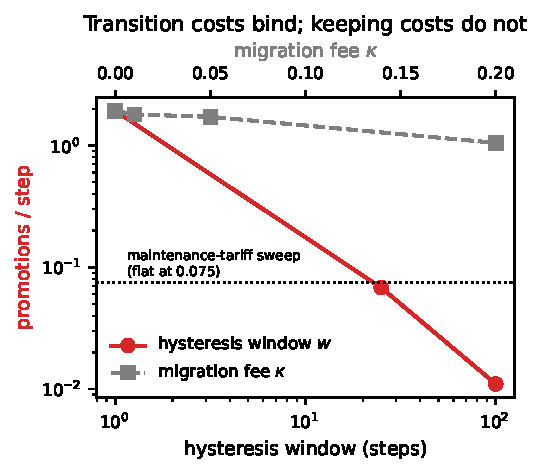
\includegraphics[width=0.62\linewidth]{figs/fig_dose_response.pdf}
\caption{Routing throughput responds to transition prices over a $175\times$ range
(hysteresis window, red; migration fee $\kappa$, gray) while maintenance tariffs leave it flat
(dotted reference). The operative price of persistence is movement, not storage.}
\label{fig:dose}
\end{figure}

\subsection{Three operating regimes}
The dose--response surface partitions behavior into saturated, selective, and frozen bands
(Fig.~\ref{fig:regimes}). In the saturated band the router moves a trace at every window opening, so
timing carries no information while trace \emph{selection} correlates with recent errors
($\approx1.15\times$ baseline). In the frozen band rare migrations anti-correlate with errors
($\approx0.52$). The selective band was tested for error-coupled timing at ten unsaturated seeds after
pre-registering a 1.05 contrast threshold: median contrast 0.97, four seeds above threshold,
one-sided $p=0.83$ --- not supported. Migration timing in this mechanism is set by price crossings
against switching costs, not by prediction errors, at every operating point we can power-test. Priced
persistence and surprise-gated memory are distinct control structures.

\begin{figure}[t]
\centering
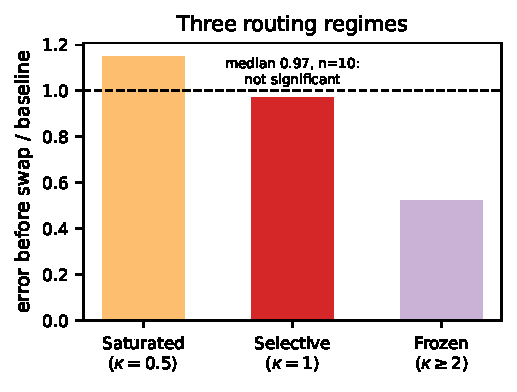
\includegraphics[width=0.55\linewidth]{figs/fig_regimes.pdf}
\caption{Error preceding migrations, relative to baseline, across the three routing regimes.
Only the saturated band shows above-baseline coupling, and there it concerns which trace moves,
not when. Selective-band timing was tested at $n=10$ and found indistinguishable from chance.}
\label{fig:regimes}
\end{figure}

\subsection{Policy comparison under the corrected router}

\begin{figure}[t]
\centering
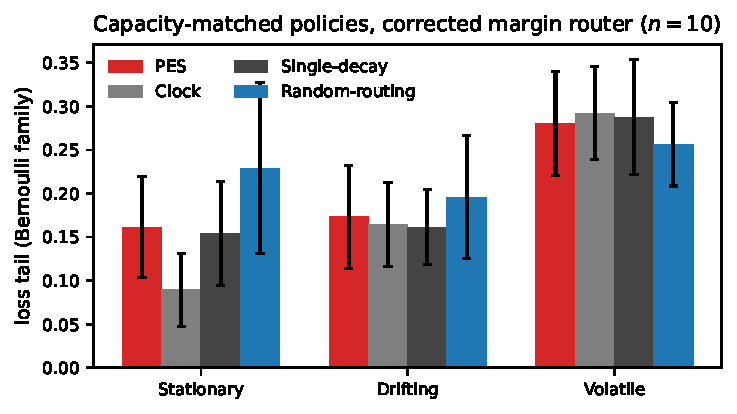
\includegraphics[width=0.85\linewidth]{figs/fig_main_comparison.pdf}
\caption{Loss tails for capacity-matched policies across regimes (Bernoulli family, $n=10$).
Exact leave-one-out pricing (red) halves the error of the same router with cheap gradient tags in
stationary retention, ties fixed-clock consolidation, stays numerically best under drift, and keeps
noise valuation strictly worst --- while all routing machinery is held fixed. Under volatile churn no
policy separates.}
\label{fig:main}
\end{figure}

Fig.~\ref{fig:main} summarizes the four-way comparison. Two structural observations survive rule
correction. First, single-store decay matches valued two-store policies under drift but loses its
protection advantage wherever retention dominates, consistent with the tariff-space reading: without a
slow store there is nothing whose loss the switching fee could have prevented. Second, random valuation
never wins a regime, which is the empirical content of value necessity.

\subsection{Ablations}
Removing any economic component individually degrades volatile-regime performance under the level-rule
implementation (tails 0.240 full $\to$ 0.270 without switching cost, 0.274 without hysteresis, 0.305
without fast decay, 0.268 without slow tariff). Under the corrected margin router the components become
redundant at these scales (all configurations within 0.280$\pm$0.06), indicating that the margin rule's
strictness already suppresses the churn those components existed to prevent. Component contributions
are therefore rule-dependent --- itself evidence that mechanism design in this space must be analyzed
jointly with the selection rule, not component-wise.

\subsection{Nonlinear port: value necessity replicates, priced routing does not}
\label{sec:nnport}
With a two-layer MLP replacing the linear predictor (stably slot-bound inputs; calibrated online
configuration), the necessity result replicated: noise valuation remained catastrophically worse than
every valued policy. Our registered hypothesis that capacity pressure would favor the priced router,
however, was falsified in the opposite direction (Fig.~\ref{fig:mlp}): tightening input capacity from
70 slots against 10 true supports to 20 slots made fixed-clock consolidation \emph{better} relative to
greedy exchange (stationary tails 0.013 vs 0.100). The diagnosis is credit misassignment: pressure
raises routing frequency exactly where first-order prices are least reliable, because
$\partial\hat y/\partial x_i$ through a tanh layer omits feature interactions. A slow clock samples the
noisy price rarely and averages the noise away. Pricing requires a trustworthy price; naive gradient
tags degrade fastest in busy markets.

A first attempt to import the linear substrate's fix --- a first-order output-side Taylor surrogate of
the deletion cost, computed through the live network --- made matters worse rather than better (tails
$0.104$ vs $0.031$ for tags vs $0.013$ for the clock; five paired seeds with identical ordering in
every pair). Pricing removal as a potential \emph{gain} demands counterfactual accuracy that a
linearization through interacting hidden units cannot supply: when the surrogate errs, it errs
precisely on the traces worth protecting. The open problem therefore stands, now bounded on both
sides --- exact prices exist only in closed-form regimes, and naive surrogates demonstrably do not
bridge the gap.

\begin{figure}[t]
\centering
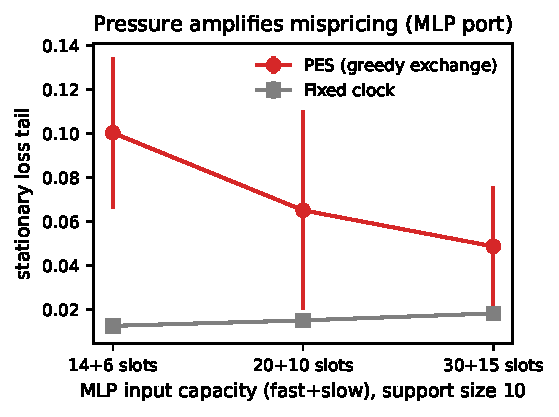
\includegraphics[width=0.6\linewidth]{figs/fig_mlp_pressure.pdf}
\caption{Capacity pressure on the MLP substrate amplifies the advantage of infrequent consolidation:
as slots approach the support size, greedy exchange with first-order prices loses to the fixed clock.}
\label{fig:mlp}
\end{figure}
\section{Discussion}
\label{sec:discussion}

The program yields one positive design principle, one confirmed prediction, and one open boundary. The
principle: persistence economics is a coherent normative frame---it derives routing from a single
priced objective, recovers established mechanisms as corners of its tariff space
(Table~\ref{tab:corners}), provably allocates optimally given prices (Propositions~\ref{prop:static},
\ref{prop:dynamic}), and exposes movement cost as the operative control knob, with a $175\times$
dose--response law and three behavioral regimes. The confirmed prediction: when the framework said the
router's deficit was a pricing problem rather than a structural one, swapping cheap gradient tags for
exact leave-one-out prices fixed it without touching any other component---halving retention error and
tying fixed-schedule consolidation. A framework earns credibility by surviving its own diagnosis, and
this one did. The open boundary: exact prices exist only where deletion effects are computable in
closed form. On the nonlinear substrate of Section~\ref{sec:nnport}, first-order tags misattribute
credit exactly when routing is most frequent, and no closed-form correction is available; making price
discovery trustworthy through nonlinearity---influence-style probes at decision moments, learned
critics, or amortized surrogates validated against exact linear prices---is the concrete next problem.
The two results are two sides of one statement: \emph{allocation is solved given honest prices;
honest price discovery beyond the linear regime is not}.

Three methodological observations generalize beyond this study. First, before interpreting when a gated
controller acts, verify its action budget is unsaturated; a saturated controller's timing describes its
budget, not its policy, and at least some published gating claims may be measuring clocks. Second,
component-wise ablation conclusions do not transfer across selection rules (Section~5.6): mechanism
components interact with the rule that consults them, so ablations should be reported per rule. Third,
pre-registration converted several of our own seductive post-hoc stories into falsifiable tests---two
of which failed---and we believe the resulting paper is stronger, not weaker, for it.

\paragraph{Limitations.} All laws are measured in vitro on sparse linear streams from one generator
lineage plus one Gaussian variant; the nonlinear port uses a two-layer MLP at moderate seed counts;
routing is greedy under additive value with no synergy analysis; value attribution is first-order; no
deep-network or language-model deployment is included; and the corrected margin router was introduced
after the initial experiments, so cross-rule comparisons, while internally consistent within each rule,
span two implementations. These limitations bound every claim above.

\section{Conclusion}

We asked whether memory hierarchy structure can be derived rather than designed. Within a priced
allocation framework the answer divides into three parts. Derivation is possible in principle: one
objective recovers known mechanisms as corner pricings and allocates provably optimally given prices.
The frame is scientifically productive: its diagnosis that routing quality tracks price quality
survived an experimental test, with exact leave-one-out pricing halving retention error and closing the
gap to fixed-schedule consolidation while machinery stayed fixed. And the frame locates its own limit:
where deletion effects cannot be priced in closed form---nonlinear predictors above all---trustworthy
price discovery replaces allocation as the binding constraint. What a learning machine should remember
is what earns its keep minus what it costs to keep; this paper contributes the accounting structure,
the evidence that honest accounting is the operative lever, and a measured statement of where the
accounting still cannot be made honest.

\paragraph{Reproducibility.}
Experiments run on numpy and matplotlib; torch appears only in Section~\ref{sec:nnport}. Twenty-three
unit tests gate every change to the core. Environment seeds derive from crc32 hashes of regime names
and are stable across machines. Every number in this paper exists in committed JSON artifacts with the
scripts that generated them; predictions and competing hypotheses were registered before their runs.
Code and artifacts accompany this paper under an MIT license.

\section*{AI use disclosure}
AI tools were used for code development assistance and manuscript review only. All experimental design,
execution, and analysis were conducted by the author using pre-registered protocols, and the author
takes full responsibility for the work.

\bibliographystyle{plainnat}
\begin{thebibliography}{30}

\bibitem[Anderson and Schooler(1991)]{anderson1991rational}
J.~R. Anderson and L.~J. Schooler.
\newblock Reflections of the environment in memory.
\newblock \emph{Psychological Science}, 2(6):396--408, 1991.

\bibitem[Ba et~al.(2016)]{ba2016using}
J.~Ba, G.~E. Hinton, D.~Kumaran, et~al.
\newblock Using fast weights to attend to the recent past.
\newblock In \emph{Advances in Neural Information Processing Systems}, 2016.

\bibitem[Behrouz et~al.(2024)]{behrouz2024titans}
A.~Behrouz, P.~Zhong, and V.~Mirrokni.
\newblock Titans: Learning to memorize at test time.
\newblock arXiv:2501.00663, 2024.

\bibitem[Behrouz et~al.(2025)]{behrouz2025nested}
A.~Behrouz, M.~Razaviyayn, P.~Zhong, and V.~Mirrokni.
\newblock Nested learning: The illusion of deep learning architectures.
\newblock In \emph{NeurIPS}, 2025. arXiv:2512.24695.

\bibitem[Benna and Fusi(2016)]{benna2016synaptic}
M.~K. Benna and S.~Fusi.
\newblock Computational principles of synaptic memory consolidation.
\newblock \emph{Nature Neuroscience}, 19:1697--1706, 2016.

\bibitem[Chen and Cheng(2026)]{chen2026learning}
Z.~Chen and Q.~Cheng.
\newblock Learning what to remember: A cognitively grounded multi-factor value model for agentic
memory.
\newblock arXiv:2606.12945, 2026.

\bibitem[Dohare et~al.(2024)]{dohare2024plasticity}
S.~Dohare, J.~Hernandez-Garcia, Q.~Lan, et~al.
\newblock Loss of plasticity in deep continual learning.
\newblock \emph{Nature}, 632:768--774, 2024.

\bibitem[Gershman(2025)]{gershman2025recallgated}
S.~Gershman et~al.
\newblock Selective consolidation of learning and memory via recall-gated plasticity.
\newblock eLife reviewed preprint 90793, 2025.

\bibitem[Graves et~al.(2014)]{graves2014neural}
A.~Graves, G.~Wayne, and I.~Danihelka.
\newblock Neural Turing machines.
\newblock arXiv:1410.5401, 2014.

\bibitem[Graves et~al.(2016)]{graves2016hybrid}
A.~Graves, G.~Wayne, M.~Reynolds, et~al.
\newblock Hybrid computing using a neural network with dynamic external memory.
\newblock \emph{Nature}, 538:471--476, 2016.

\bibitem[Hinton and Plaut(1987)]{hinton1987fast}
G.~E. Hinton and D.~C. Plaut.
\newblock Using fast weights to deblur old memories.
\newblock In \emph{Proceedings of the Ninth Annual Conference of the Cognitive Science Society}, 1987.

\bibitem[Kaplanis et~al.(2018)]{kaplanis2018complex}
C.~Kaplanis, M.~Shanahan, and M.~Clopath.
\newblock Continual reinforcement learning with complex synapses.
\newblock In \emph{ICML}, 2018.

\bibitem[Kirkpatrick et~al.(2017)]{kirkpatrick2017ewc}
J.~Kirkpatrick, R.~Pascanu, N.~Rabinowitz, et~al.
\newblock Overcoming catastrophic forgetting in neural networks.
\newblock \emph{PNAS}, 114(13):3521--3526, 2017.

\bibitem[Li et~al.(2026{\natexlab{a}})]{li2026duallayer}
W.~Li et~al.
\newblock Dual-layer agentic memory with fast write routing and slow consolidation.
\newblock arXiv:2608.22215, 2026.

\bibitem[Li(2026{\natexlab{b}})]{li2026ngc}
M.~Li.
\newblock Neural garbage collection: Learning to forget while learning to reason.
\newblock arXiv:2604.18002, 2026.

\bibitem[Schlag et~al.(2021)]{schlag2021linear}
I.~Schlag, K.~Irie, and J.~Schmidhuber.
\newblock Linear transformers are secretly fast weight programmers.
\newblock In \emph{ICML}, 2021.

\bibitem[Sun et~al.(2024)]{sun2024testtime}
Y.~Sun, X.~Li, K.~Dalal, et~al.
\newblock Learning to (learn at test time): {RNNs} with expressive hidden states.
\newblock arXiv:2407.04620, 2024.

\bibitem[Veeriah et~al.(2021)]{veeriah2021discovery}
V.~Veeriah, M.~Ryzhov, G.~Tucker, et~al.
\newblock Discovery of useful questions and alternative gradient estimators for learned optimizers.
\newblock arXiv:2011.02159, 2021.

\bibitem[Yang et~al.(2024)]{yang2024gated}
S.~Yang, B.~Wang, Y.~Zhang, et~al.
\newblock Gated delta networks: Improving {Mamba2} with delta rule.
\newblock arXiv:2412.06464, 2024.

\bibitem[Zenke et~al.(2017)]{zenke2017si}
F.~Zenke, B.~Poole, and S.~Ganguli.
\newblock Continual learning through synaptic intelligence.
\newblock In \emph{ICML}, 2017.

\bibitem[Zhang et~al.(2025)]{zhang2025obcache}
Z.~Zhang et~al.
\newblock {OBCache}: Optimal brain {KV} cache pruning for efficient long-context {LLM} inference.
\newblock arXiv:2510.07651, 2025.

\end{thebibliography}

\appendix

\section{Reproducibility details}
\label{app:repro}
Environment parameters: $D{=}200$ inputs, support $s_0{=}25$, noise $\sigma{=}0.05$, common-coordinate
probability mass $0.8$, rare-factor $30$; Bernoulli family draws $x_i\sim\mathrm{Bern}(p_i)\cdot
\mathcal N(0,1)$, Gaussian family draws $x_i\sim\mathcal N(0,0.5)$ masked to the support. Regime
parameters: stationary $p_{\mathrm{ch}}=0$; drifting $p_{\mathrm{ch}}=0.002$; volatile
$p_{\mathrm{ch}}=0.01$; alternating swaps two frozen rules every $T/4$ steps. Learner: linear predictor
$\hat y = w^\top x_A$ over active set $A$; SGD $\eta=0.15$; value EMA $\rho=0.98$; capacities
$(45,15)$; maturity gate 50 steps; default $\kappa=0.02$, hysteresis 25. MLP port: 64 hidden units,
tanh, online Adam at $3\times10^{-3}$ with gradient clipping 1.0, stable input-slot binding. Every run
records loss tails (last 20\%), promotion/eviction ledgers, and per-trace residence snapshots into
versioned JSON artifacts.

\end{document}
